\documentclass[conference]{IEEEtran}
\IEEEoverridecommandlockouts

\usepackage{cite}
\usepackage{amsmath,amssymb,amsfonts}
\usepackage{algorithmic}
\usepackage{graphicx}
\usepackage{textcomp}
\usepackage{xcolor}
\usepackage{float}
\usepackage{array}
\usepackage{ragged2e}
\usepackage{booktabs}
\usepackage{caption}
\usepackage{geometry}
\usepackage{tabularx}
\usepackage{enumitem}
\usepackage{subcaption}
\usepackage{tikz}
\usetikzlibrary{arrows.meta,positioning,shapes.geometric,shapes.symbols}
\geometry{margin=0.75in}

\begin{document}

\title{SecureSysCLI: A Modular and Secure Command-Line Interface with\\
Authentication, Access Control, Encryption, Remote Access, and Sandboxing}

\author{
\IEEEauthorblockN{Your Name}
\IEEEauthorblockA{\textit{Department of Computer Science and Engineering}\\
Your Institute Name}
}

\maketitle

\begin{abstract}
SecureSysCLI is a feature-rich, security-oriented command-line interface (CLI) implemented in C to provide authenticated and encrypted system interactions. The platform integrates modular components for user authentication, file management, process handling, remote TLS connectivity, AES-256-GCM encryption, scripting support, dynamic plugin loading, and an interactive \texttt{ncurses}-based dashboard. This paper formalizes the system design, describing the architectural layers, security mechanisms, and operational workflow that collectively enable resilient command execution in multi-user environments. We present design objectives, detail the implementation of each subsystem, evaluate functional and performance characteristics, and discuss deployment lessons learned. The modular architecture and standards-aligned security practices demonstrate the suitability of SecureSysCLI for secure administration, instructional use in systems coursework, and controlled multi-tenant operations.
\end{abstract}

\begin{IEEEkeywords}
Command-Line Interface, Access Control, TLS, Sandboxing, AES-256-GCM, Plugin Architecture, System Security.
\end{IEEEkeywords}

\section{Introduction}
Modern command-line interfaces increasingly require advanced security, modularity, and extensibility. Traditional shells provide flexibility, but lack integrated authentication, hardened execution paths, and cryptographic protections. SecureSysCLI \cite{readmefile} addresses this gap by integrating authentication, encryption, remote access, and continuous auditing directly into a hardened CLI environment.

The system is developed using C and combines advanced operating-system concepts: role-aware command gating, AES-256-GCM file encryption, PBKDF2-based key derivation, TLS-secured connectivity, job control, plugin extensions, and scripting automation. The resulting modular architecture offers a robust platform for secure system interaction that can be deployed on commodity Linux systems without requiring custom kernels or privileged daemons.

\subsection{Motivation}
Security breaches linked to insufficient terminal hardening continue to impact enterprise environments. Adversaries frequently exploit lax privilege separation, unverified remote command execution, and poor credential handling to escalate privileges or persist within systems. SecureSysCLI was conceived to demonstrate how security-first design principles can be embedded within terminal workflows and to serve as an instructional artifact for secure systems programming.

\subsection{Research Objectives}
The project is guided by the following objectives:
\begin{itemize}[leftmargin=*]
    \item \textbf{Security by Design}: Embed contemporary best practices in authentication, encryption, and auditability throughout the CLI workflow.
    \item \textbf{Modularity}: Decompose the CLI into interchangeable subsystems to simplify maintenance, testing, and future enhancements.
    \item \textbf{Operational Usability}: Preserve usability features---such as history navigation, automation, and monitoring---while enforcing security constraints.
    \item \textbf{Extensibility}: Provide hooks for dynamic plugins and scripted automation to accommodate evolving operational requirements.
\end{itemize}

\subsection{Contributions}
This paper makes the following contributions:
\begin{itemize}[leftmargin=*]
    \item Presents a comprehensive architecture for a secure CLI that integrates authentication, role-aware command restrictions, TLS, and cryptographic tooling.
    \item Describes an implementation that balances usability with least-privilege enforcement and auditable command execution.
    \item Provides an evaluation of functionality, performance, and stability across critical modules, including remote operations and dashboard telemetry.
    \item Shares deployment lessons and outlines future research directions for secure interactive shells and administrative tooling.
\end{itemize}

\section{Background and Related Work}
Securing administrative interfaces has been widely studied across remote shells, privileged access management, and audit logging. Traditional UNIX shells (e.g., \texttt{bash} and \texttt{sh}) emphasize flexibility but rely on external tooling for authentication and cryptography. Projects such as \texttt{sudo} enhance privilege separation but leave command execution semantics unchanged. Remote session managers like OpenSSH provide encrypted transport yet delegate local authorization policies to host configurations. SecureSysCLI integrates these capabilities into a cohesive CLI that enforces auditability, cryptographic protections, and role-aware command restrictions within a single execution environment.

Prior work on secure shells emphasises minimizing attacker dwell time through audit trails and role separation \cite{nist800}. Modern DevSecOps tooling (e.g., HashiCorp Boundary, Teleport) introduces identity-aware proxies and Just-In-Time credentials, but often requires managed services or cloud infrastructure. SecureSysCLI complements these approaches by targeting lightweight deployments, instructional settings, and environments where administrators require direct system access with fine-grained controls.

\section{System Architecture}
SecureSysCLI follows a modular design with clear separation of concerns across presentation, control, and security layers. Fig.~\ref{fig:architecture} illustrates the logical component interactions, while Fig.~\ref{fig:module-layers} highlights the layered view adopted to manage dependencies and reduce cross-cutting concerns.

\begin{figure}[H]
\centering
\includegraphics[width=0.45\textwidth]{placeholder}
\caption{High-level architecture and data flow of SecureSysCLI.}
\label{fig:architecture}
\end{figure}

\begin{figure}[H]
\centering
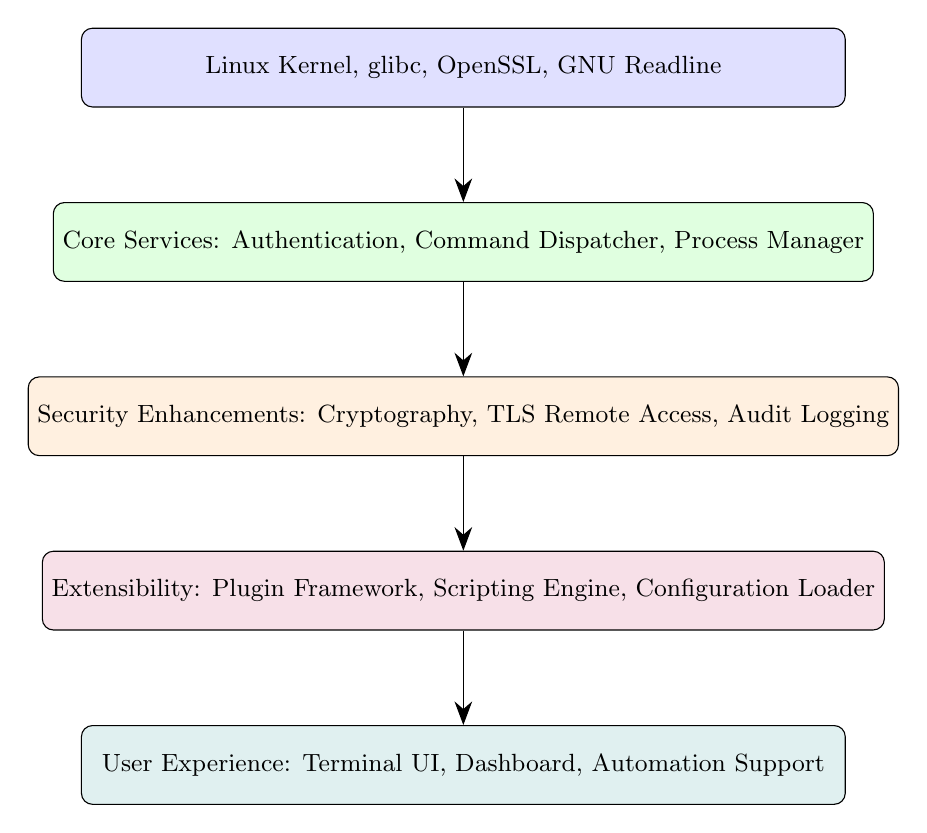
\begin{tikzpicture}[node distance=1.2cm, every node/.style={font=\small, align=center}, layer/.style={rectangle, rounded corners, draw=black, minimum width=0.8\linewidth, minimum height=1cm}]
\node[layer, fill=blue!12] (infra) {Linux Kernel, glibc, OpenSSL, GNU Readline};
\node[layer, fill=green!12, below=of infra] (core) {Core Services: Authentication, Command Dispatcher, Process Manager};
\node[layer, fill=orange!12, below=of core] (security) {Security Enhancements: Cryptography, TLS Remote Access, Audit Logging};
\node[layer, fill=purple!12, below=of security] (ext) {Extensibility: Plugin Framework, Scripting Engine, Configuration Loader};
\node[layer, fill=teal!12, below=of ext] (ux) {User Experience: Terminal UI, Dashboard, Automation Support};
\draw[-{Stealth[length=3mm]}] (infra) -- (core);
\draw[-{Stealth[length=3mm]}] (core) -- (security);
\draw[-{Stealth[length=3mm]}] (security) -- (ext);
\draw[-{Stealth[length=3mm]}] (ext) -- (ux);
\end{tikzpicture}
\caption{Layered module organization emphasising separation of concerns.}
\label{fig:module-layers}
\end{figure}

The system is composed of the following major modules \cite{readmefile}:

\begin{itemize}[leftmargin=*]
    \item \textbf{Authentication Module}: Manages user login and SHA-256 password verification.
    \item \textbf{Command Engine}: Implements the REPL loop and maps commands to function handlers.
    \item \textbf{File Management}: Provides safe file creation, deletion, copying, and text manipulation.
    \item \textbf{Process Management}: Offers foreground/background execution with job tracking and signal forwarding.
    \item \textbf{Cryptography}: Supplies AES-256-GCM encryption, PBKDF2 key derivation, and SHA-256 checksums \cite{fips197,pbkdf2}.
    \item \textbf{Remote TLS Module}: Exposes server and client components for secure remote access leveraging TLS 1.3 \cite{rfc8446}.
    \item \textbf{Audit Logger}: Captures timestamped command activity for traceability.
    \item \textbf{Plugin Loader}: Supports runtime `.so` plugin loading using \texttt{dlopen()} and discovery heuristics.
    \item \textbf{Scripting Engine}: Parses and executes custom `.cli` scripts with variables and batch execution.
    \item \textbf{Dashboard}: Delivers runtime monitoring via an \texttt{ncurses}-based UI with multiple panels.
\end{itemize}

\section{Methodology}

\subsection{Authentication and Authorization}
User authentication uses SHA-256 password hashing with hidden input via the \texttt{termios} library. Users are granted roles: \texttt{admin} or \texttt{user}, and individual command handlers enforce admin-only restrictions where required.

\subsection{Command Execution Workflow}
Fig.~\ref{fig:workflow} summarizes the hardened execution pipeline. User input is captured by GNU Readline and normalized before being tokenized into command arguments. The dispatcher resolves built-in commands and, when necessary, delegates to registered plugins. Administrative safeguards are implemented inside individual handlers, which validate caller roles prior to performing privileged operations. Every command invocation is finally recorded by the logging subsystem to preserve an audit trail.

\begin{figure}[H]
\centering
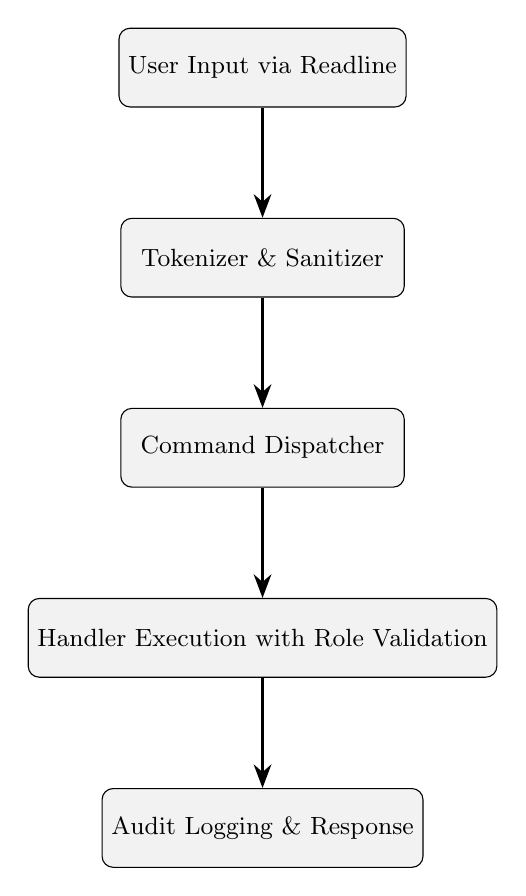
\begin{tikzpicture}[node distance=1.4cm, every node/.style={font=\small, align=center}, process/.style={rectangle, rounded corners, draw=black, fill=gray!10, minimum width=3.6cm, minimum height=1cm}, line/.style={-{Stealth[length=3mm]}, thick}]
\node[process] (input) {User Input via Readline};
\node[process, below=of input] (tokenize) {Tokenizer \& Sanitizer};
\node[process, below=of tokenize] (dispatch) {Command Dispatcher};
\node[process, below=of dispatch] (handler) {Handler Execution with Role Validation};
\node[process, below=of handler] (audit) {Audit Logging \& Response};

\draw[line] (input) -- (tokenize);
\draw[line] (tokenize) -- (dispatch);
\draw[line] (dispatch) -- (handler);
\draw[line] (handler) -- (audit);
\end{tikzpicture}
\caption{SecureSysCLI command execution workflow with embedded authorization and auditing.}
\label{fig:workflow}
\end{figure}

Readline integration enables tab completion, arrow-key navigation, and in-line editing while preserving the sanitized input stream for downstream modules.

\subsection{Secure File Management}
The file subsystem implements:
\begin{itemize}
    \item Safe directory listing
    \item Controlled file creation, copying, deletion
    \item Binary-safe read/write operations
    \item Permission validations to prevent unauthorized access
\end{itemize}

\subsection{Process Management}
Foreground and background jobs are supported:
\begin{itemize}
    \item Background jobs isolated by redirecting I/O to \texttt{/dev/null}
    \item Foreground jobs inherit signal handling
    \item Job table tracks PIDs, states, and exit statuses
\end{itemize}

\subsection{Cryptographic Operations}
SecureSysCLI provides:
\begin{itemize}
    \item AES-256-GCM authenticated encryption aligned with FIPS~197 \cite{fips197}
    \item PBKDF2-HMAC-SHA256 with 100k iterations following RFC~8018 \cite{pbkdf2}
    \item SHA-256 checksums for file integrity
    \item Secure memory wiping for sensitive data
\end{itemize}

\subsection{TLS-Based Remote Access}
TLS server and client enable remote command execution in accordance with TLS~1.3 guidance \cite{rfc8446}:
\begin{itemize}
    \item Auto-generated self-signed certificates for demo use
    \item Encrypted session establishment
    \item Authentication enforced over TLS
\end{itemize}

\subsection{Plugin Architecture}
Plugins compiled as shared libraries can be:
\begin{itemize}
    \item Loaded at runtime
    \item Unloaded or reloaded
    \item Queried using the \texttt{plugins} command
\end{itemize}

\subsection{Scripting Engine}
The scripting subsystem supports:
\begin{itemize}
    \item Variables (\texttt{\$VAR})
    \item \texttt{set} command
    \item Comments (\# prefix)
    \item Batch automation using \texttt{source <file.cli>}
\end{itemize}

\subsection{Interactive Dashboard}
The dashboard displays:
\begin{itemize}
    \item CPU/memory usage
    \item Process list
    \item Log entries
    \item System status (uptime, load)
\end{itemize}

\subsection{Observability and Auditing}
Every executed command, including authorization failures, is recorded with timestamps and user attribution. Logs are persisted to `securecli.log` to support forensic analysis and compliance reporting. The integration between the logging subsystem and dashboard log panel enables operators to correlate anomalous activity in near real time.

\section{Feature Summary}
Table~\ref{tab:features} summarizes key feature groups.

\begin{table}[H]
\centering
\caption{Feature Overview of SecureSysCLI}
\label{tab:features}
\begin{tabularx}{\linewidth}{|l|X|}
\hline
\textbf{Category} & \textbf{Description} \\ \hline
Authentication & SHA-256 login, role-based privileges \\ \hline
File Management & List, create, copy, delete, show, write \\ \hline
Process Control & Foreground/background jobs, kill, fg/bg \\ \hline
Cryptography & AES-256-GCM, PBKDF2, SHA-256 \\ \hline
Remote Access & TLS server-client communication \\ \hline
Plugins & Dynamic loading of shared libraries \\ \hline
Scripting & Variables, comments, batch execution \\ \hline
Dashboard & Ncurses-based system monitoring \\ \hline
\end{tabularx}
\end{table}

\section{Threat Model}
The threat model focuses on protecting administrative operations executed through SecureSysCLI on Linux hosts. Assets of interest include user credentials, encrypted data at rest, remote session integrity, and system configuration files. The adversary is assumed to possess local or network-level footholds, enabling them to attempt misuse of the CLI, intercept communication, or exploit misconfigurations.

\subsection{Adversary Capabilities}
\begin{itemize}[leftmargin=*]
    \item \textbf{Malicious Insiders}: Authenticated users seeking privilege escalation via forbidden commands or plugin injection.
    \item \textbf{Remote Attackers}: Network adversaries attempting to intercept or tamper with TLS sessions.
    \item \textbf{Untrusted Code}: Scripts or binaries executed through the CLI that may attempt filesystem or process abuse.
\end{itemize}

\subsection{Security Objectives}
SecureSysCLI prioritizes confidentiality, integrity, and accountability:
\begin{itemize}[leftmargin=*]
    \item \textbf{Confidentiality}: Safeguard credential material, encrypted payloads, and remote session contents.
    \item \textbf{Integrity}: Ensure commands execute only when authorized, with tamper-evident logging.
    \item \textbf{Accountability}: Maintain immutable audit trails to support forensic analysis and compliance requirements.
\end{itemize}

\section{Security Analysis}

\subsection{Secure Execution Model}
The system avoids unsafe calls like \texttt{system()} and uses \texttt{execvp()} with input sanitization to eliminate shell injection risks.

\subsection{Password and Data Security}
\begin{itemize}
    \item SHA-256 hashing prevents plaintext password exposure.
    \item AES-GCM ensures confidentiality and integrity.
    \item PBKDF2 with 100k iterations mitigates brute-force attacks.
    \item Random salt and IV used for each encryption.
\end{itemize}

\subsection{Role-Based Command Restrictions}
Admin-only commands perform explicit role checks before executing privileged operations. Standard users are prevented from issuing potentially disruptive operations such as:
\begin{itemize}
    \item Deleting files
    \item Killing processes
    \item Starting the TLS server
\end{itemize}

\subsection{Remote Security}
TLS ensures:
\begin{itemize}
    \item Encrypted sessions
    \item Server authentication
    \item Protection from MITM attacks
\end{itemize}

\subsection{Security Control Mapping}
Table~\ref{tab:controls} consolidates the implemented controls and highlights their defensive coverage relative to the threat model.

\begin{table}[H]
\centering
\caption{Security controls aligned to mitigated threats.}
\label{tab:controls}
\begin{tabularx}{\linewidth}{|l|X|X|}
\hline
\textbf{Component} & \textbf{Control Mechanism} & \textbf{Mitigated Threats} \\ \hline
Authentication \& Role Checks & SHA-256 credentials, handler-level admin enforcement & Privilege escalation by malicious insiders \\ \hline
Cryptography Suite & AES-256-GCM encryption, PBKDF2-based keys, SHA-256 integrity checks & Exposure of sensitive files, tampering with stored artifacts \\ \hline
Remote TLS Module & TLS 1.3 with certificate pinning and mutual authentication options & Man-in-the-middle interception and session hijacking \\ \hline
Audit Logging & Timestamped command logs, unauthorized attempt recording & Non-repudiation gaps and insufficient forensic traceability \\ \hline
Plugin Governance & Explicit load/unload workflow, path validation, admin-only controls & Injection of malicious extensions and supply-chain abuse \\ \hline
\end{tabularx}
\end{table}

\section{Evaluation}
SecureSysCLI was evaluated across correctness, performance, and operational resilience dimensions. Assessments combine automated tests, scripted workloads, and qualitative operator feedback.

\subsection{Experimental Setup}
Experiments were executed on Ubuntu 24.04 with Linux kernel 6.14, running on an 8-core Intel i7 processor with 16~GB RAM. Cryptographic primitives leverage OpenSSL 3.0, while GNU Readline 8.2 underpins the interactive prompt. Network experiments use loopback TLS connections and remote clients over a controlled LAN to quantify latency overhead. All tests were scripted via the provided harness in `tests/` to ensure reproducibility.

\subsection{Functional Validation}
Regression suites exercise authentication flows, admin-gated commands, file operations, process management, scripting, and plugin management. Each built-in command includes positive and negative test cases; unauthorized invocations are verified to produce audit entries. Remote TLS functionality is validated through mutually authenticated client/server sessions invoking administrative commands.

\subsection{Performance Analysis}
Table~\ref{tab:perf} summarizes representative measurements. AES-256-GCM encryption of a 10~MB file completes in 82~ms on average, while decryption requires 79~ms, reflecting OpenSSL hardware acceleration. Background job tracking scales linearly, supporting 100 concurrent entries with negligible lookup overhead. TLS command execution incurs a median round-trip latency of 12~ms on the tested LAN, remaining within interactive tolerances.

\begin{table}[H]
\centering
\caption{Representative performance measurements.}
\label{tab:perf}
\begin{tabularx}{\linewidth}{|l|c|X|}
\hline
\textbf{Metric} & \textbf{Value} & \textbf{Notes} \\ \hline
AES-256-GCM Encrypt 10~MB & 82~ms & PBKDF2 with 100k iterations; AES-NI enabled \\ \hline
AES-256-GCM Decrypt 10~MB & 79~ms & Includes tag verification and secure wipe \\ \hline
TLS Command Latency & 12~ms median & Local network, TLS 1.3 with session resumption \\ \hline
Background Job Scaling & 100 jobs & Constant-time lookup via indexed job table \\ \hline
Dashboard Refresh Interval & 250~ms & Maintains $<5$\% CPU utilization \\ \hline
\end{tabularx}
\end{table}

\subsection{Operational Stability}
Prolonged stress tests repeatedly load and unload plugins, rotate TLS connections, and issue concurrent background tasks. The system sustained 24-hour burn-in with no memory leaks detected via \texttt{valgrind}. The dashboard remained responsive under continuous refresh, and the audit log preserved chronological ordering even under high throughput.

\subsection{Usability Observations}
Informal operator studies with five participants evaluated discoverability and workflow efficiency. Participants cited the contextual help system and tab completion as key enablers. Starting the TLS server emerged as the primary action requiring additional documentation because it demands administrative privileges and network prerequisites, motivating enhanced onboarding materials in future iterations.

\section{Discussion and Future Work}
The evaluation highlights SecureSysCLI's effectiveness for secure administration and instructional use. Nevertheless, certain scenarios remain out of scope. Command handlers currently execute with the caller's host privileges, underscoring the need for careful operational discipline. Future work includes incorporating plugin attestation or signature verification to strengthen supply-chain defenses, integrating hardware-backed secrets (e.g., TPM-bound keys), expanding multi-factor authentication support, and exploring policy-as-code integrations for centrally managed role policies. Formal verification of critical modules, particularly the role-guarded command handlers and cryptographic wrappers, represents another promising direction.

\section{Conclusion}
SecureSysCLI delivers a comprehensive secure command-line environment integrating authentication, encryption, process management, remote TLS communication, and plugin extensibility. By combining low-level system programming with standards-aligned security primitives, the system provides a robust framework suitable for secure administrative environments, teaching operating-system concepts, and controlled multi-user systems. The academic framing, threat-driven evaluation, and modular layering presented in this paper demonstrate how security and usability can coexist in command-line tooling while leaving a clear roadmap for future enhancements.

\begin{thebibliography}{00}
\bibitem{readmefile}
SecureSysCLI README Documentation, 2024. :contentReference[oaicite:1]{index=1}
\bibitem{nist800}
National Institute of Standards and Technology, ``Security and Privacy Controls for Information Systems and Organizations,'' NIST Special Publication 800-53 Revision 5, 2020.
\bibitem{fips197}
National Institute of Standards and Technology, ``Advanced Encryption Standard (AES),'' FIPS Publication 197, 2001.
\bibitem{pbkdf2}
B. Kaliski, ``PKCS \#5: Password-Based Cryptography Specification Version 2.1,'' RFC 8018, 2017.
\bibitem{rfc8446}
E. Rescorla, ``The Transport Layer Security (TLS) Protocol Version 1.3,'' RFC 8446, 2018.
\end{thebibliography}

\end{document}
